% ============================================================
%  §2  Intuitive Picture
% ============================================================

\section{Intuitive Picture}
\label{sec:intuitive}

Before introducing the formal apparatus, we sketch the intuitive picture
that motivates the technical development.

\subsection{Thought as Movement Across Terrain}

Consider the experience of working through a difficult problem.
Some directions of thought feel natural and low-cost; others require
effort and tend to be abandoned.
Some ideas return repeatedly without deliberate intention; others, once
visited, leave no trace.
The experience of ``understanding'' something is not the acquisition of
a new object, but a change in the ease with which one can move through
a region of thought.

These observations suggest a spatial metaphor: thought moves across a
terrain whose shape is not fixed in advance but is formed by the
history of prior movement.
Frequently traversed paths become smoother; regions that are never
visited grow inaccessible.
The terrain itself is invisible to the traveler, who experiences only
the ease or difficulty of each step.

This is the intuitive core of Conceptual Topography.
Figure~\ref{fig:potential-geometry} summarizes this geometric picture.

\begin{figure}[t]
  \centering
  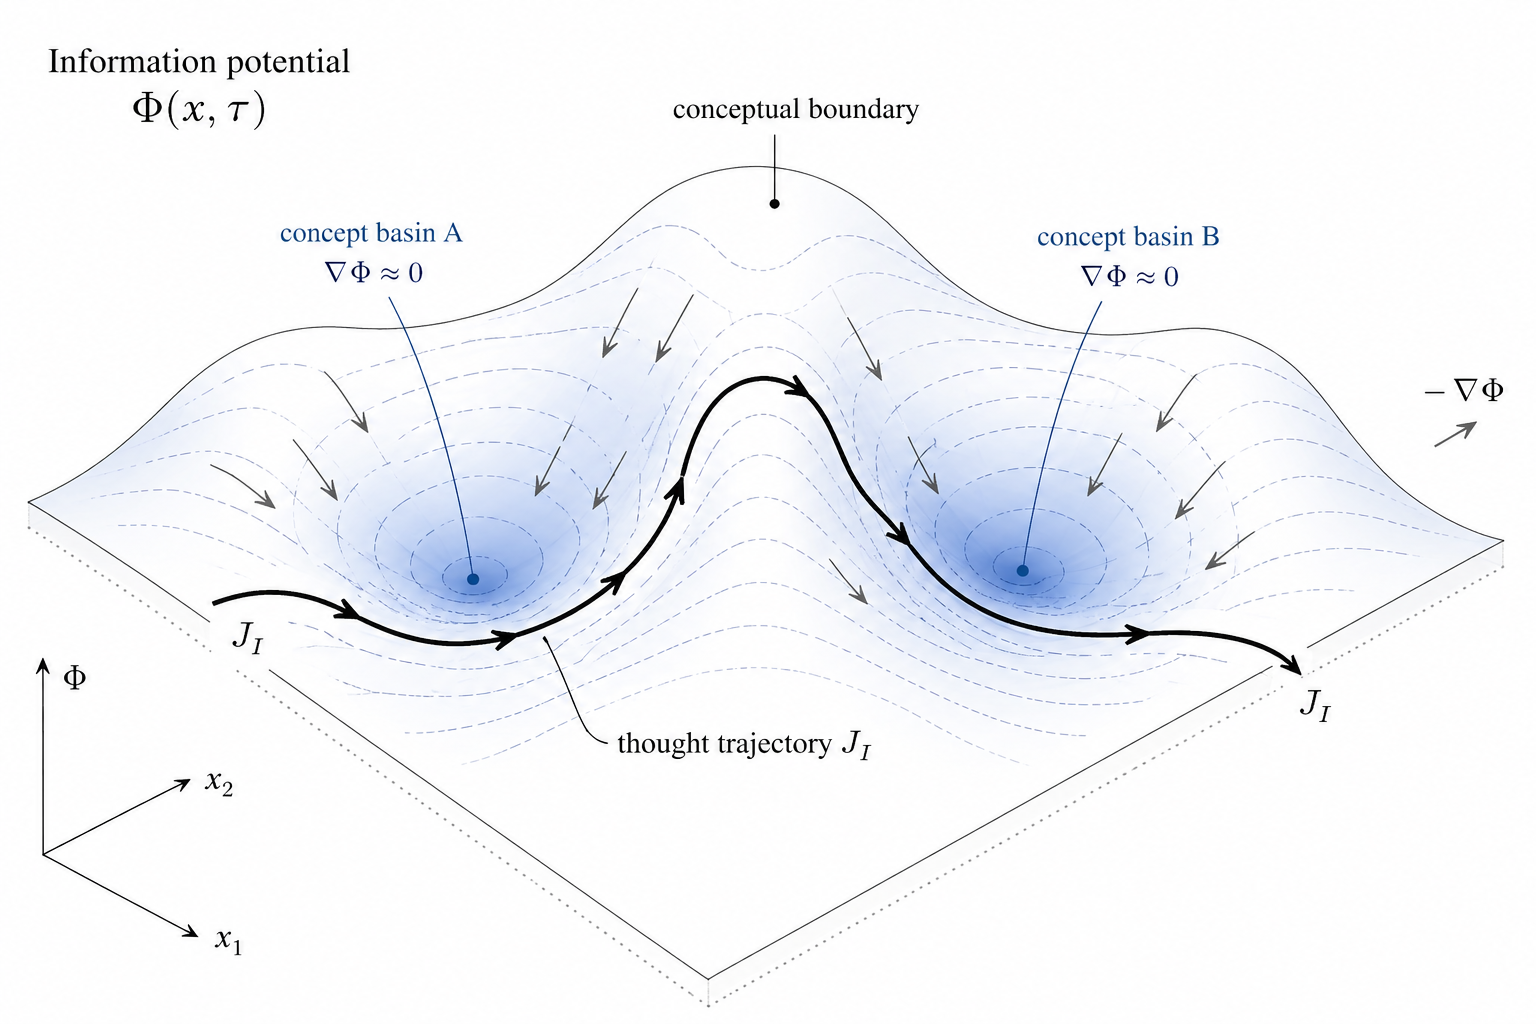
\includegraphics[width=0.92\linewidth]{figures/fig1_potential_geometry.png}
  \caption{
  Conceptual landscape as information-potential geometry.
  The surface represents the information potential $\Phi(x,\tau)$.
  Concepts correspond to locally stable basins where $\nabla\Phi \approx 0$.
  Thought is represented as the trajectory of information flow $J_I$ constrained by the gradient structure of the landscape.
  Ridges correspond to high-cost conceptual boundaries.
  }
  \label{fig:potential-geometry}
\end{figure}

The ``terrain'' is the information potential $\Phi(x,\tau)$, shaped by
the accumulated history of information flow $\JI$.
The ``movement'' is the trajectory of $\JI$ along $-\nabla\Phi$.
The ``understanding'' is a local reduction in $|\nabla\Phi|$
in a previously difficult region.

\subsection{Concepts as Valleys}

In this picture, a concept is a valley in the potential landscape:
a region of low $\Phi$ toward which trajectories are naturally drawn.
The depth of the valley reflects how frequently the corresponding
region has been traversed; its width reflects the range of contexts
in which the concept applies.

Crucially, the valley does not contain a meaning.
It is a \emph{dynamical attractor}: a region of the field that
systematically draws in subsequent trajectories and makes certain
patterns of thought more likely.
What we call the ``meaning'' of a concept is, in this framework,
the set of trajectories that the attractor makes available.

\subsection{Linguistic Tokens as Terrain-Shaping Operations}

Linguistic tokens --- understood broadly to include not only natural
language words but any discrete, re-addressable medium capable of acting
on the field as a localized perturbation: symbols, emblems, gestures,
diagrams, mathematical notation, and so on --- do not carry meanings
from speaker to listener.
They act as localized perturbations that shift the potential landscape
slightly toward or away from existing attractors.
When a discrete unit is used repeatedly in similar contexts, it deepens
the associated valley; when it falls out of use, the valley shallows.
Communication succeeds not because meanings are transferred, but because
sender and receiver have sufficiently similar landscape geometries
that the same perturbation produces similar trajectory shifts.

\subsection{The Invisible GPU}

The landscape operates below the threshold of conscious access.
Thought moves across the terrain, but the terrain itself is not
represented or inspected during movement.
This gives rise to the characteristic phenomenology of cognition:
the sense that certain thoughts ``come naturally,'' that certain
connections ``suggest themselves,'' that understanding arrives
suddenly rather than being constructed step by step.

These experiences reflect the geometry of $\Phi$, not the content of
any represented meaning.

The formal development in subsequent sections makes these intuitions
precise.
